\begin{figure}[ht!]
	\centering
	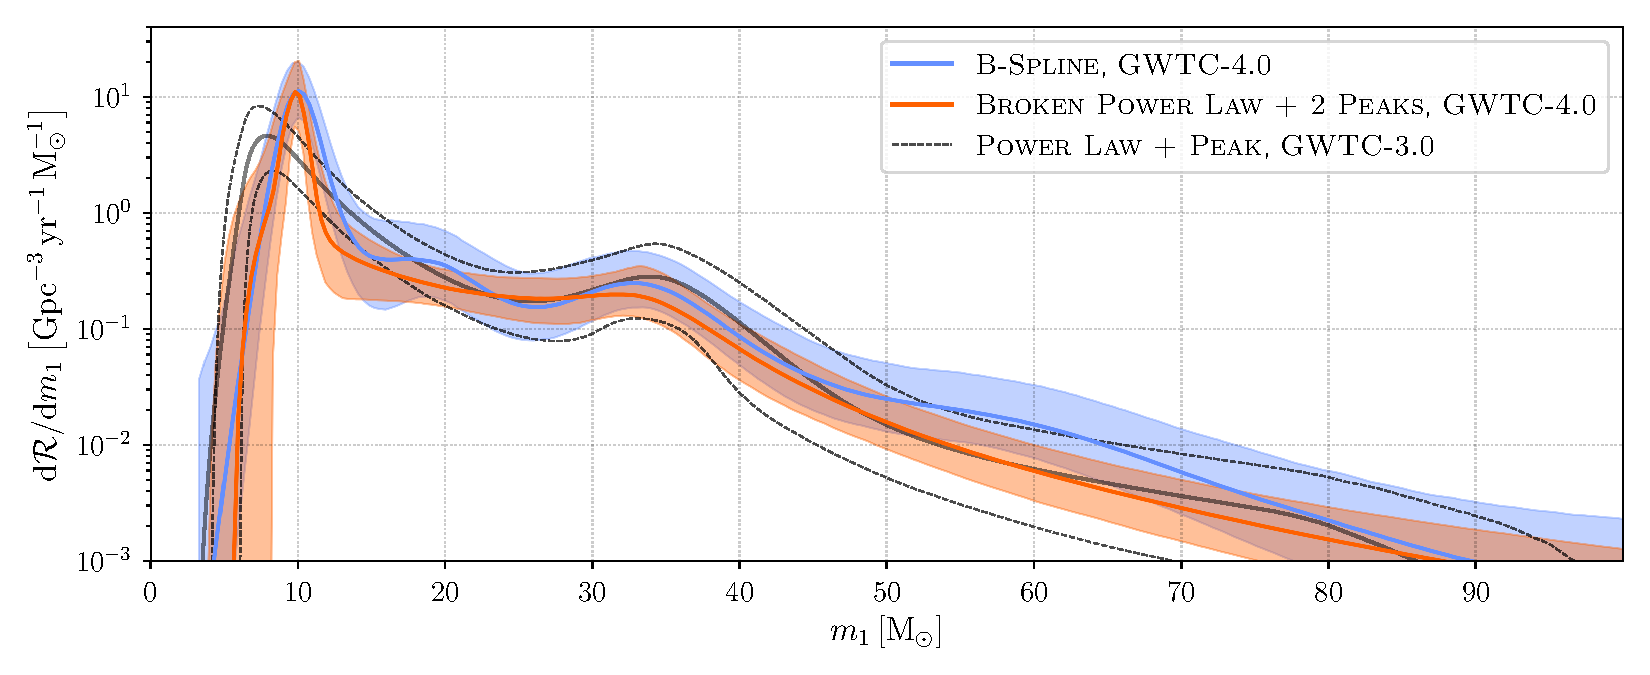
\includegraphics[width=\textwidth]{figures/primary_mass_default.pdf}
	\caption{Differential merger rate as a function of primary mass (evaluated at $z=0.2$) of the \BrokenPLTwoPeaks model (orange) and \BSpline model (blue) compared to the \PLPeak model from \gwtcthree \citep{KAGRA:2021duu}. The solid lines indicate the posterior medians and the shaded regions show the 90\% credible interval of each model. Comparing these results, it is clear that a single power law is a poor description of the the low-mass end of the spectrum.}
	\label{fig:primary_mass_default}
  \end{figure}
  
\section{Binary Black Hole Population}\label{sec:bbh_results}
In this section, we analyze the astrophysical population of \acp{BBH} using data from \ac{GW} events with a \ac{FAR} $< 1 \,\text{yr}^{-1}$. We only include events whose $1\%$ lower limit on both component mass posteriors (under the \ac{PE} priors) is larger than $3 \, \Msun$.
There are {$\counts[FAROnePerYear][O4aBBH]$} events from \ac{O4a} that meet this criterion in addition to the $69$ \ac{BBH} events from \gwtcthree, which brings the total number of \ac{BBH} events passing our \ac{FAR} threshold to {$\counts[FAROnePerYear][totalBBH]$}. Of the events considered in \ac{O4a}, only GW230529 does not meet this criterion and is not considered in the analyses below (see Section~\ref{sec:data}).



%%%%%%%%%%%%%%%%%%%%%%%%
\subsection{Primary Mass}
%%%%%%%%%%%%%%%%%%%%%%%%
\label{subsec:bbh_masses}

In this section, we illustrate the main findings of the strongly and weakly modeled approaches using results from the \BrokenPLTwoPeaks (see Appendix \ref{appendix:BrokenPLTwoPeaks}) and \BSpline (see Appendix \ref{appendix:BSpline}) models, respectively. We chose the \BrokenPLTwoPeaks model as our fiducial mass model because it performed the best in our model comparison study. It was first introduced by \citet{Callister:2023tgi} to describe the \gwtcthree mass distribution. Results from a selection of other models considered in the model comparison study can be found in Appendix \ref{appendix:model_comparison_mass}, while models that employ a \nonparametric can be found in Appendix \ref{appendix:non_parameteric_comparison}, both of which include comparisons to the fiducial \BrokenPLTwoPeaks and \BSpline models. The \parametric employs the default models listed in Table \ref{tab:summary_of_models} for the other source parameters, namely the \powerlawRedshift and \default models.

\textbf{We identify a global peak at $\bm{{\sim}10 \,\Msun}$ and find that it is robust to model variations}. A Gaussian-like peak at ${\sim}10 \,\Msun$ was first identified by \citet{Tiwari:2020otp} and \citet{Edelman:2021zkw} using \gwtctwo and later by the \nonparametrics in \citet{KAGRA:2021duu} using \gwtcthree. Figure \ref{fig:primary_mass_default} shows the rate ${\rm d}\mathcal{R}/{\rm d} m_1$ as a function of primary mass at $z=0.2$ inferred by these models compared to the \PLPeak (see Appendix B of \citealt{KAGRA:2021duu} for a description of this model) inference with \gwtcthree from \citet{KAGRA:2021duu}.\footnote{We quote \ac{BBH} merger rates at $z=0.2$ to be consistent with \citet{KAGRA:2021duu} and because $z\sim0.2$ is where we best constrain the merger rate.} The low-mass Gaussian component of the \BrokenPLTwoPeaks model infers a global peak in the primary mass spectrum at $m_1 = \CIPlusMinus{\defaultbbh[mass_1][peak_1_location]} \,\Msun$ relative to the underlying broken power law continuum. The \BSpline model also recovers a global peak at $m_1 = \CIPlusMinus{\BsplineIID[mass_1][peak_1_location]} \,\Msun$. Both values are consistent with \gwtcthree, which inferred a global peak at $m_1 = $ \muOOT by modeling the mass spectrum as a power law modulated by a spline.

\textbf{A broken power law is necessary to describe the continuum structure above $\bm{{\sim}15 \,\Msun}$} (see Figure \ref{fig:primary_mass_default}). Below ${\sim}35 \, \Msun$, the continuum  of \ac{BH} masses is well described by a power law with spectral index $\alpha_1 = \CIPlusMinus{\defaultbbh[alpha_1]}$. Above ${\sim}35 \, \Msun$, the continuum steepens, with a spectral index of $\alpha_2 = \CIPlusMinus{\defaultbbh[alpha_2]}$ that is consistent with the \PLPeak result from \gwtcthree ($\alpha = $ \alphaOT). We find that $\alpha_2 > \alpha_1$ at $\defaultbbh[alpha_diff_perc] \%$ credibility. Though this continuum structure was identified by \citet{Callister:2023tgi}, it was not identified by the \parametrics in \citet{KAGRA:2021duu}, in part due to the limited flexibility of models employed in \citet{KAGRA:2021duu}. To illustrate this, in Figure \ref{fig:primary_mass_o3b_comparison} we present a re-analysis of \gwtcthree using the \BrokenPLTwoPeaks model alongside the \gwtcfour result, which shows improved constraints across the full mass spectrum. 

\textbf{We identify a feature at $\bm{{\sim}35\, \Msun}$}. Using the \parametric, we find that this feature is consistent with either: (i) an over-density that peaks at $m_1 = \CIPlusMinus{\defaultbbh[mass_1][peak_2_location]} \, \Msun$ relative to an underlying broken power law (i.e., the \BrokenPLTwoPeaks result), or (ii) a broken power law with break mass $m_\text{break} = \CIPlusMinus{\PowerLawTwoPeakOneBBH[break_mass]} \,\Msun$ (i.e., a broken power law without a second peak near the break). See Appendix \ref{appendix:model_comparison_mass} for a more detailed discussion of this result. The former conclusion is supported by the \BSpline model, which exhibits a local peak at $m_1 = \CIPlusMinus{\BsplineIID[mass_1][peak_2_location]} \,\Msun$, consistent with other models that employ a \nonparametric in Appendix \ref{appendix:non_parameteric_comparison}. 

\textbf{Additional structure may be present in the mass spectrum}. A bump near ${\sim}20 \,\Msun$ is present in some of the \nonparametrics (see Figure \ref{fig:bbh_mass_non_parametrics} in Appendix \ref{appendix:non_parameteric_comparison}). We cannot conclude with the \parametric whether adding a third Gaussian component to the \BrokenPLTwoPeaks model in this region is required by the data or not (as quantified by the log Bayes factor $\log_{10}\mathcal{B} = \BBHMassModelBayesFactors[pl2pk3]$ between the default model and one including a third peak). This feature was first reported in an analysis of \gwtctwo \citep{Tiwari:2020otp} and was present in several analyses of \gwtcthree \citep{KAGRA:2021duu,Edelman:2022ydv, Tiwari:2023xff,Godfrey:2023oxb}. Additionally, the \BSpline and other \nonparametrics show a rise in the merger rate relative to the \BrokenPLTwoPeaks result in the ${\sim}60 \,\Msun$ region, which can be seen in Figure \ref{fig:primary_mass_default} and Figure \ref{fig:bbh_mass_non_parametrics}. A previous study of \gwtcthree found evidence for a similar feature in this region \citep{MaganaHernandez:2024qkz}.


\begin{figure*}[t]
	\centering
	\includegraphics[width=0.9\linewidth]{figures/fig_primary_mass_default_comparison.pdf}
	\caption{Differential merger rate as a function of primary mass (evaluated at $z=0.2$) of the \BrokenPLTwoPeaks model inferred with \gwtcfour compared to the same model applied to only \gwtcthree \ac{BBH} events. The orange shaded region shows the 90\% credible interval for \gwtcfour and the solid orange curve shows the posterior median, while the black dashed curves bound the $90\%$ credible region for \gwtcthree and the solid black curve shows the posterior median. The inferred distribution is similar between catalogs, which highlights that the low-mass structure identified in \gwtcfour was present in \gwtcthree. The inset figure shows the joint posterior of the broken power law index parameters $\alpha_1$ and $\alpha_2$ for \gwtcthree (gray) and \gwtcfour (orange), with the contours showing the $5^{\rm th}, 50^{\rm th}$, and $95^{\rm th}$ percentiles. The black dashed curve in the inset indicates where $\alpha_1 = \alpha_2$.}
	\label{fig:primary_mass_o3b_comparison}
  \end{figure*}

We do not place informative constraints on the individual parameters that govern low-mass smoothing for the \BrokenPLTwoPeaks model. We caution against astrophysically interpreting the \ac{BBH} primary mass distribution below ${\sim} 8 \,\Msun$ because of the bias that may be introduced by removing the probable \ac{NS}-containing events in the manner described in Section~\ref{sec:data}. Removing such events is responsible for the discrepancy below ${\sim} 8 \,\Msun$ between Figure \ref{fig:full_mass_spectrum} and Figure \ref{fig:primary_mass_default}.

\gwtcfour includes an exceptional high-mass BBH, GW231123~\citep{GW231123}, whose inferred component masses lie at the extreme upper end of those in our dataset. To check if GW231123 is an outlier with respect to the mass distribution of \acp{BBH}, we construct mock catalogs containing $153$ detected events following the inferred population without GW231123, and calculate the distribution of maximum detectable \ac{BH} masses. The total mass of GW231123 lies at the $\CIPlusMinus{\OutlierTestMassiveEvent[percentilemmax300][total_mass_source]}$th percentile of this distribution. This shows that while GW231123 lies in the tail of the distribution, its total mass is consistent with the inferred mass spectrum; the degree of consistency is more than was the case with \gwtcthree data alone~\citep{GW231123}.

The main compact binary formation scenarios (\citealt{{Mandel:2018hfr}} and references therein)---isolated binary evolution and dynamical assembly in dense stellar environments---have both been shown to produce populations consistent with current observations \citep{Mandel:2021smh}. A peak near $m_1 \sim 10 \, \Msun$ is often predicted by isolated binary evolution models \citep{Dominik:2014yma, Belczynski:2017gds, Giacobbo:2018etu, Wiktorowicz:2019dil, Neijssel:2019irh}, while mass distributions from dynamical formation, such as in young and globular clusters, typically peak above $10\, \Msun$ \citep{Rodriguez:2016kxx, Hong:2018bqs, Rodriguez:2019huv, Banerjee:2020qub, Antonini:2020xnd}. However, predictions from isolated and dynamical formation often overlap and can vary significantly based on the assumptions and methodologies used, making it difficult to conclude the origin of the observed catalog or constrain formation physics based on features in the marginal mass distributions. 

A feature that may provide distinguishing power between the isolated and dynamical channels is the existence of an upper mass gap, in the range $45\,\Msun \lesssim m \lesssim 120 \,\Msun$. Such a dearth would be consistent with the theorized \textit{pair-instability mass gap}, arising from the complete disruption of massive stars due to runaway electron--positron pair production \citep{Woosley:2016hmi,Mapelli:2019ipt,Farmer:2019jed}. While the precise locations of the lower and upper edges of the pair-instability mass gap are sensitive to physical assumptions \citep{Renzo:2020rzx, vanSon:2020zbk, Woosley:2021xba, Shen:2023rco, Winch:2024xdt}, the feature tends to be a robust prediction of most stellar evolution models \citep{Marchant:2018kun,Marchant:2020haw,Renzo:2020rzx,Woosley:2021xba}. The gap may not be completely empty due to overmassive stellar envelope fallback or stellar mergers \citep{DiCarlo:2019pmf, DiCarlo:2019fcq, Mapelli:2019ipt, Kremer:2020wtp}, hierarchical BBH mergers in clusters or in AGN environments \citep{Mckernan:2017ssq, Rodriguez:2019huv, McKernan:2019beu, Yang:2019okq, Mapelli:2020xeq, Antonini:2018auk, Fragione:2020nib, Liu:2020gif, Martinez:2020lzt, Sedda:2020jvg, Mahapatra:2021hme, Mahapatra:2022ngs, Mahapatra:2024qsy}, or even due to primordial \acp{BH} \citep{Postnov:2014tza, Bird:2016dcv, Clesse:2020ghq}. The decrease in the merger rate above $m_1 \sim35 \, \Msun$ seen in all models and the tentative rise near $m_1\sim60 \, \Msun$ seen in the \nonparametrics may hint toward a polluted mass gap.


\begin{figure}
	\centering
	\includegraphics[width=0.9\columnwidth]{figures/mass_ratio_default.pdf}
	\caption{Differential merger rate as a function of mass-ratio (evaluated at $z=0.2$) of the \BrokenPLTwoPeaks model (orange) and \BSpline model (blue). The fiducial \textsc{Power Law + Peak} model from \citet{KAGRA:2021duu} is included for comparison. Solid curves indicate posterior medians and the shaded (dashed) regions show 90\% credible intervals.}
	\label{fig:mass_ratio_default}
  \end{figure}


\subsection{Mass-Ratio}
\label{subsec:bbh_ratio}

Figure \ref{fig:mass_ratio_default} shows the differential merger rate ${\rm d}\mathcal{R}/{\rm d}q$ evaluated at $z = 0.2$ inferred by the \BrokenPLTwoPeaks and \BSpline models compared to the \PLPeak result from \gwtcthree.\footnote{Models that utilize B-Splines infer the separable distribution $p(q)$ but the results of such models shown in this section are actually the conditional marginal distribution $p(q|m_2{>}3\Msun)$. See Appendix \ref{appendix:BSpline} for further details.}

\textbf{We find that the mass-ratio distribution can be described by a power-law with an index $\bm{\beta_q = \CIPlusMinus{\defaultbbh[beta]}}$} that is consistent with \gwtcthree ($\beta_q = 1.1^{+1.7}_{-1.3}$) with a reduction in uncertainty. The \BSpline model shows a reduced rate above $q \gtrsim 0.8$ relative to the \BrokenPLTwoPeaks result. More flexible parametrizations in the \parametric were explored (see also the other \nonparametrics in Figure \ref{fig:bbh_mass_non_parametrics}, which do peak near unity), but model comparisons were inconclusive. Similarly, in \gwtcthree, \citet{Godfrey:2023oxb} inferred a mass-ratio distribution peaked away from unity using a \nonparametric, while \citet{Rinaldi:2025emt} found equal evidence for two \parametrics with very distinct behavior above $q \gtrsim 0.7$. 

Models that incorporate correlations between source parameters have a greater potential to distinguish between formation channels than uncorrelated ones. We next present results from two different models that correlate features of the primary mass spectrum with different mass-ratio distributions. 

\textbf{\acp{BH} with masses $\bm{{\sim} 35\, \Msun}$ preferentially merge with other \acp{BH} of more equal mass relative to those in the underlying mass continuum.} The \ExtendedBrokenPLTwoPeaks model modifies the \BrokenPLTwoPeaks model by allowing each primary mass mixture component (i.e., the broken power law and two Gaussian components) to be associated with a different power-law-mass-ratio distribution. Figure \ref{fig:mass_ratio_peak} shows the mass-ratio distribution for each mixture component. Specifically, each component infers a different power-law index $\beta_q$, with $\beta_q^{\rm BP} = \CIPlusMinus{\VaryingBetaQsDominantMode[param][beta_q_power_law]}$ for the broken power law, $\beta_q^{\rm peak1} = \CIPlusMinus{\VaryingBetaQsDominantMode[param][beta_q_low_mass_peak]}$ for the Gaussian component that captures the ${\sim}10\, \Msun$ peak, and $\beta_q^{\rm peak2} = \CIPlusMinus{\VaryingBetaQsDominantMode[param][beta_q_high_mass_peak]}$ for the second Gaussian component that captures the ${\sim}35 \, \Msun$ feature. Critically, $\beta_q^{\rm peak2} > \beta_q^{\rm BP}$ at $\VaryingBetaQsDominantModeBetaDiffPerc[beta_peak_pl_diff_perc] \%$ credibility. See Appendix \ref{appendix:model_comparison_mass} for a more detailed discussion of this result. Other studies of \gwtcthree have drawn similar conclusions about the pairing preferences of high mass \acp{BH} \citep[e.g., ][]{Li:2022jge, Baibhav:2022qxm, Sadiq:2023zee, Galaudage:2024meo, Roy:2025ktr}. 

\textbf{\acp{BH} with masses $\bm{{\sim}10\, \Msun}$ may prefentially merge with lighter \acp{BH}}. The region bounded by the solid blue curves in the bottom panel of Figure \ref{fig:mass_ratio_peak} shows the mass-ratio distribution of the ${\sim}10 \,\Msun$ peak inferred with the \textsc{Isolated Peak} model. This model is a mixture of a Gaussian peak and a B-Spline (continuum) in primary mass, and the mass ratio and spin distributions are inferred separately for each mixture component with B-Splines (see Appendix \ref{appendix:non_parametric_models_summary} for further details). The Gaussain peak is inferred at ${\sim}10 \,\Msun$ and its mass-ratio distribution exhibits a peak at $q = \CIPlusMinus{\IsoPeakIID[mass_ratio][peak][peak_location]}$, a feature that a single power law is unable to reproduce. This could explain the large uncertainty in $\beta_q^{\rm peak1}$ from the \ExtendedBrokenPLTwoPeaks model. The solid blue curve in Figure \ref{fig:mass_ratio_peak} shows the mass-ratio distribution of masses outside of the ${\sim}10 \,\Msun$ peak inferred by the B-Spline mixture component. Unlike the full population mass-ratio distribution inferred by the \BSpline model in Figure \ref{fig:mass_ratio_default}, this result does not possess a peak near $q \sim 0.8$, indicating that the peak seen in the full population is due largely to the events around ${\sim}10 \,\Msun$. This mass feature was identified in \gwtcthree by \citet{Godfrey:2023oxb}. 

\begin{figure}[t]
	\centering
	  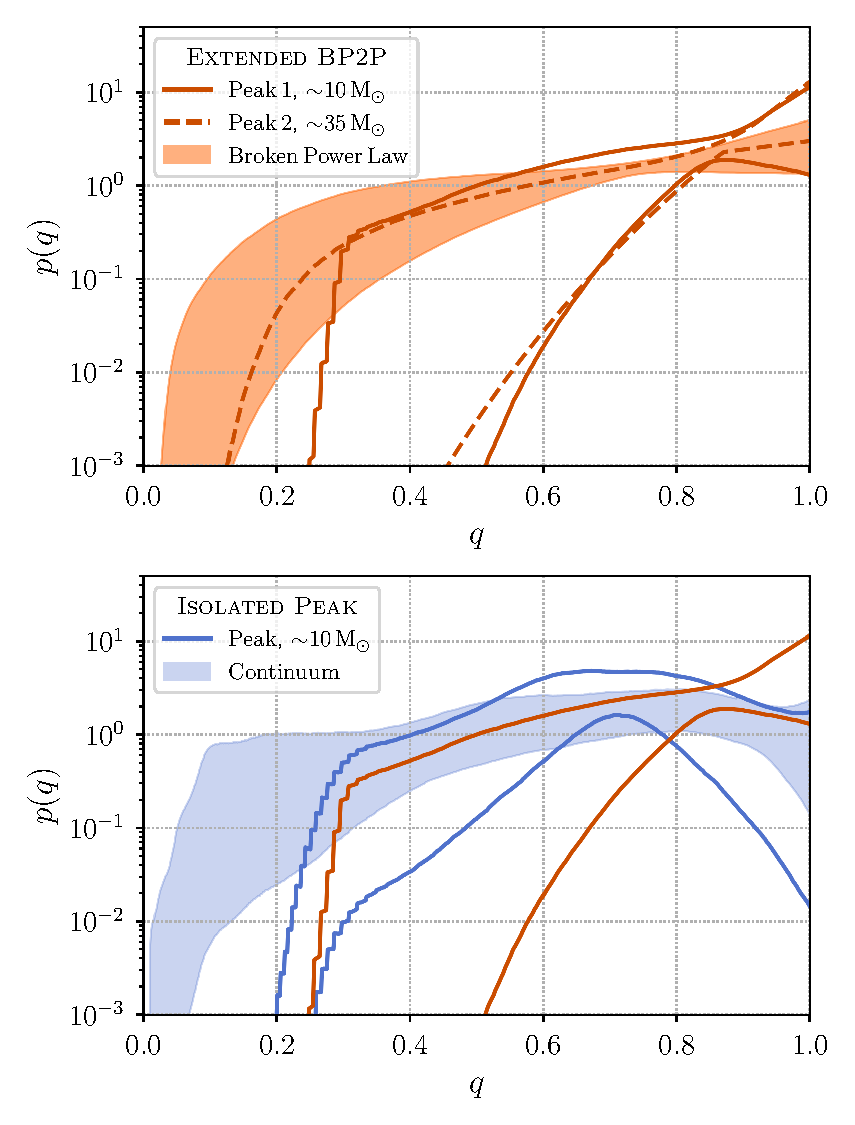
\includegraphics[width=0.6\columnwidth]{figures/fig_mass_ratio_peak.pdf}
	  \caption{Top Panel: The $90\%$ credible regions for the mass-ratio distribution of the ${\sim}10 \,\Msun$ peak (solid orange curves), ${\sim}35 \,\Msun$ peak (dashed curves), and continuum (orange shaded region) components of the \ExtendedBrokenPLTwoPeaks model. Bottom Panel: The $90\%$ credible regions for mass-ratio distribution of the ${\sim}10 \,\Msun$ peak (solid blue curves) and the rest of the mass spectrum (blue shaded region) inferred with the \textsc{Isolated Peak} model. The ${\sim}10\, \Msun$ peak mass-ratio distribution from the \ExtendedBrokenPLTwoPeaks is included for comparison.}
	  \label{fig:mass_ratio_peak}
  \end{figure}

Most formation channels generally favor equal mass systems. For example, dynamical formation can produce systems with a wide range of mass ratios, but predicted distributions typically peak at unity \citep{Rodriguez:2016kxx, Torniamenti:2024uxl}. Certain hierarchical mergers may not necessarily follow this trend, in particular mergers between first generation and second generation BHs have been shown to produce a mass-ratio distribution peaked near $q \sim 0.5$ \citep{Rodriguez:2019huv}. Mass transfer during the contact phase of binaries formed via chemically homogeneous evolution~\citep{deMink:2016vkw, Marchant:2016wow} leads to a strong preference for equal mass-ratio systems, but this mechanism is thought to be important for binaries with $\massone \gtrsim 10\,\Msun$~\citep{duBuisson:2020asn, Zevin:2020gbd, Riley:2020btf}. Mass-ratio reversal within the stable mass transfer channel can lead to a peak in the mass-ratio distribution between $q\sim$ 0.6-0.8 \citep{Neijssel:2019irh,vanSon:2021zpk}, which is qualitatively consistent with the mass-ratio distribution of the ${\sim}10 \,\Msun$ inferred with the \textsc{Isolated Peak} model. Stable mass transfer also predicts a peak near ${\sim}10 \,\Msun$ that is robust to uncertainties in the metallicity-dependent star formation history \citep{vanSon:2022ylf} and other physical uncertainties of the channel \citep{vanSon:2022myr}.
%%%%%%%%%%%%%%%%%%%%%%%%
\subsection{Spin}
%%%%%%%%%%%%%%%%%%%%%%%%
\label{subsec:bbh_spins}

We next present the spin distribution of the \ac{BBH} population through O4a.
We model spins using two different parameterizations: the magnitudes $\chi_i$ and tilt angles $\theta_i$ (Section~\ref{subsubsec:bbh_spin_mag_and_tilts}), and the effective inspiral spin $\chieff$ and effective precessing spin $\chip$ (Section~\ref{subsubsec:bbh_effective_spins}).
The effective inspiral spin $\chieff$ is the mass-weighted average of the component spins \textit{aligned} with the binary's orbital angular momentum~\citep{Racine:2008qv,Ajith:2009bn}.
The effective precessing spin $\chip$ characterizes the degree of relativistic precession caused by spin--orbit misalignment, capturing the effect of the \textit{in-plane} spin components~\citep{Schmidt:2010it,Schmidt:2012rh,Schmidt:2014iyl,Gerosa:2020aiw}; these are defined in Equations 15 and 16 of \cite{GWTC:Introduction}.
More details about spin parameterization are given in Appendix~\ref{appendix:spinModels}.

Previous analyses of the \acp{BBH} observed through O3 found that \ac{BH} spin vectors tend to be small in magnitude ($\chi\lesssim 0.3$) and preferentially---but not exclusively---lie above the orbital plane \citep[$\cos\theta>0$;][]{LIGOScientific:2018jsj,LIGOScientific:2020kqk,KAGRA:2021duu}. 
The new observations in \gwtcfour further support these conclusions and additionally suggest more structure in the component and effective spin distributions, enabled by changes to the models used in previous population analyses:
(i) \textbf{the spin magnitude distribution has support at $\bm{\chi\approx 0}$}, (ii) \textbf{the spin tilt distribution may peak away from perfect alignment with the orbital angular momentum}, and (iii) \textbf{the $\bm{\chieff}$ distribution is asymmetric about its peak}.
We elaborate upon these new features in the following subsections.


%%%%%%%%%%%%%%%%%%%%%%%%%%%%%%%%%%%%%%%%%%%%%%%%
\subsubsection{Spin Magnitudes and Tilts}
\label{subsubsec:bbh_spin_mag_and_tilts}
%%%%%%%%%%%%%%%%%%%%%%%%%%%%%%%%%%%%%%%%%%%%%%%%


\begin{figure*}
  \centering
  \includegraphics[width=\linewidth]{figures/spins/spin_magnitudes_and_tilts.pdf}
  \caption{Marginal spin magnitude $\chi$ (left) and cosine tilt angle $\cos\theta$ (right) distributions under the \default (blue) and \BSpline (green) models.
  The results from the \gwtcthree~{\sc Default} are shown for comparison (black dashed); note that this model is different from what is used for \gwtcfour.
  The \gwtcthree analysis employed a Beta distribution for spin magnitudes rather than a truncated normal, and fixed the location of the Gaussian component of the spin tilt angle distribution to $\cos\theta=1$ rather than letting it vary freely in inference. 
  The solid lines show the median of the inferred distributions from \gwtcfour, and the shaded regions show their 90\% credible regions.
  The thick dashed lines show the median from \gwtcthree, while the thin dashed lines show its 90\% credible region.}
  \label{fig:spin_mag_tilt_pdf}
\end{figure*}
%

Spin magnitudes and tilt angles provide insight about \ac{BBH} formation and evolution~\citep[e.g.,][]{Mandel:2018hfr,Mapelli:2018uds}; we begin with spin magnitudes.
If angular momentum transport in stars is efficient, stellar cores rotate slowly, resulting in small spin magnitudes for isolated \acp{BH}~\citep{Fuller:2019sxi,Ma:2019cpr,Fuller:2019ckz}.
However, binary interactions can significantly influence \ac{BH} spins through mechanisms such as tides~\citep{Hut:1981,Packet:1981,Zaldarriaga:2017qkw,Qin:2018vaa,Bavera:2020inc,Mandel:2020lhv} and accretion~\citep{Hut:1981,Packet:1981,vandenHeuvel:2017pwp,Neijssel:2019irh,Steinle:2020xej,Stegmann:2020kgb}. 
If a \ac{BBH} forms from a pre-existing isolated stellar binary, tidal interactions can spin up the progenitor of the second-born \ac{BH}~\citep{Bavera:2020inc,Qin:2018sxk}, yielding spin magnitudes of $\chi\approx 0.2{-}0.4$~\citep{Ma:2023nrf}, although these can be reduced by stellar winds~\citep{Tout:1992}.
Chemically homogeneous evolution---involving tidally locked, high-mass, low-metallicity, close binaries---may produce even larger spins~\citep{Mandel:2015qlu,deMink:2016vkw}. 
Alternatively, large spin magnitudes may point toward a hierarchical merger origin, where one or both \acp{BH} are remnants of previous \ac{BBH} mergers~\citep{Rodriguez:2019huv,Zhang:2023fpp,Doctor:2019ruh,Kimball:2020opk,Payne:2024ywe,Gerosa:2021mno,Fishbach:2017dwv,Gerosa:2017kvu,Mould:2022ccw,Mahapatra:2021hme,Mahapatra:2022ngs,Mahapatra:2024qsy}, which are predicted to have $\chi \sim 0.7$~\citep{Lousto:2009mf}.

With this astrophysical context, we present our measurement of the spin magnitude distribution through O4a. 
The left column of Figure~\ref{fig:spin_mag_tilt_pdf} shows the marginal distributions of $\chi$ using the \parametric~(\default; blue) and \nonparametric~(\BSpline; green).
The \default~model (Equation \ref{eqn:spin_mag_model}) describes the $\chi$ population as a truncated Gaussian distribution.
This is a departure from the {\sc Default} spin model of \gwtcthree.
There, a non-singular Beta distribution was used~\citep{KAGRA:2021duu}, which forces $p(\chi)=0$ at $\chi=0,1$ and thus cannot measure contributions to the population at near-minimal or near-maximal spins.
Allowing for more model flexibility at the $\chi$ distribution's boundaries is crucial, as there exists an ongoing discussion in the literature about whether or not there is an over-density of \acp{BBH} with $\chi \lesssim 0.01$~\citep{Kimball:2020opk,Galaudage:2021rkt,Callister:2022qwb,Tong:2022iws,Mould:2022xeu,Hussain:2024qzl}.
We find that the \default~model is preferred over the {\sc Default} spin model of \gwtcthree by $\log_{10} {\cal B} = \spinModelComparisonLogTenBayesFactors[MagTruncnormIidTiltIsotropicTruncnormNid][log10_bayes_factor_over_old_default]$; additional parametric spin magnitude (and tilt) models are discussed in Appendix~\ref{appendix:model_comparison_spins}.
The widening of the 90\% credible regions for the $\chi$ and $\cos\theta$ distributions at their boundaries under the \BSpline~model seen in Figure \ref{fig:spin_mag_tilt_pdf} is a prior-driven effect common in spline modeling \citep[e.g.,][]{Golomb:2022bon,Edelman:2022ydv}.

\textbf{In \gwtcfour, we constrain $\bm{p(\chi\approx 0) > 0}$ under both the strongly and weakly modeled approaches.}
At 90\% credibility, our recovered spin magnitude distribution peaks between $\chi=\CIBoundsDash{\MagTruncnormIidTiltIsotropicTruncnormNid[param][mu_chi]}$, as measured by the $\mu_{\chi}$ location parameter.
Broadly, \ac{BH} spins are inferred to be predominantly non-extremal, with the \default~model finding that $90\%$ of \acp{BH} having $\chi<\MagTruncnormIidTiltIsotropicTruncnormNid[ppd][a][90th percentile]$.
The comparative dearth of observed \acp{BBH} with large spins disfavors a population dominated by second-generation \acp{BH}. 
However, the precise fraction of systems with large spin magnitudes is model dependent: the \default and \BSpline models only disagree at 90\% credibility for $\chi > \defaultVersusBSplineSpinMagnitudes[chi at discrepancy=90]$.
At $\chi = 0.8$, $0.9$, and $1.0$, their $p(\chi)$ distributions differ at the $\defaultVersusBSplineSpinMagnitudes[discrepancy percentile for chi=0.8]$\%, $\defaultVersusBSplineSpinMagnitudes[discrepancy percentile for chi=0.9]$\%, and $\defaultVersusBSplineSpinMagnitudes[discrepancy percentile for chi=1.0]$\% levels, respectively.
While the \default model approaches $p(\chi)\sim 0$ at $\chi=1$,
the \BSpline~model infers a larger, nearly flat distribution from $\chi=0.6$ to $1$. 
Similar behavior was found in \gwtcthree~\citep{Godfrey:2023oxb}, and attributed to a subpopulation with near-uniform spin magnitudes.
The discrepancy between our two models may arise from limited flexibility in the \parametric; a single truncated Gaussian cannot increase the probability at $\chi \gtrsim 0.8$ without also increasing it at $\chi\sim 0.2{-}0.5$. 
In \gwtcfour, a handful of events do have preferentially large spin magnitudes, including GW231123 which has primary spin $\chi_1 > 0.5$ with high confidence~\citep{GW231123}.

Under both the \default and \BSpline models, the results presented in Figure~\ref{fig:spin_mag_tilt_pdf} assume that the spin magnitudes are \ac{IID}, meaning that the function describing the population distribution is factorizable in terms of $\chi_1$ and $\chi_2$, and the two are described by the same set of hyperparameters.
The data prefer identically distributed spin magnitudes over those which are non-identically distributed, cf.~Table~\ref{tab:modelComparisonSpins}.
However, mathematically, the primary and secondary spins cannot be \ac{IID} if the purported correlation between $q$ and $\chieff$ is true~\citep{Farr:2025}. 
We probe this correlation in Section~\ref{subsubsec:mass_spin_correlations}, and find support for its existence, albeit with evidence that has diminished since \gwtcthree. 
Thus, we interpret the Bayes factor in favor of \ac{IID} spins as a statement that, under the \default~model, we cannot yet say with statistical certainty that the spins are not identically distributed. 
This statement is likely driven by the fact that individual-event spin magnitude posterior distributions are typically wide, making $\chi_1$ and $\chi_2$ hard to distinguish. 
In general, $\chi_1$ and $\chi_2$ are not expected to be identically distributed in nature; if $q$ and $\chieff$ are indeed correlated, more informative $\chi_i$ measurements may eventually reveal their non-identical nature.
Figure~\ref{fig:spin_mags_tilts_comparison_cornerplot} in Appendix~\ref{appendix:model_comparison_spins} presents posteriors on the \default hyperparameters under the assumption that spin magnitudes (and tilts) are identically versus non-identically distributed.

%
\begin{figure}
  \centering
  \includegraphics[width=0.6\linewidth]{figures/spins/spin_sorting_traces.pdf}
  \caption{Larger ($\chi_A$, darker blue) and smaller ($\chi_B$, lighter blue) spin magnitude distributions, derived from imposing order statistics on the \default $\chi$ distribution shown in Figure~\ref{fig:spin_mag_tilt_pdf}.
  The solid lines show the median of each inferred distribution, and the shaded regions show the 90\% credible intervals.}
  \label{fig:spin_sorting_pdf}
\end{figure}
%

Next, Figure~\ref{fig:spin_sorting_pdf} shows the inferred spin magnitude distributions if, rather than sorting by the more versus less massive \ac{BH}, we instead sort by the \ac{BH} with the larger (subscript A) and smaller (subscript B) spin magnitude~\citep{Biscoveanu:2020are}. 
The magnitudes $\chi_A$ and $\chi_B$ are derived quantities and are not fit independently:
to generate their distributions, we take results from the \default~model and impose order statistics, assuming that $\chi_A$ is the larger of two draws from the $p(\chi)$ distribution in the left panel of Figure~\ref{fig:spin_mag_tilt_pdf} and $\chi_B$ is the smaller~\citep{KAGRA:2021duu, Biscoveanu:2020are}.
This analysis does not assume any sort of pairing function between spins.
Spin sorting offers an alternative way to visualize and interpret the spin information from the \ac{IID} model.
The more rapidly spinning component has a wide spin magnitude distribution, with a \ac{PPD} peaking at $\chi_A = \MagTruncnormIidTiltIsotropicTruncnormSpinSorting[ppd][chi_A][spin at peak]$, and support up to $\chi_{A,99\%}= \CIPlusMinus{\MagTruncnormIidTiltIsotropicTruncnormSpinSorting[param][chi_A_99th]}$ (value of $\chi_A$ at which each $p(\chi_A)$ trace reaches its 99th percentile, serving as a proxy for the distribution's maximum).
The vanishing probability at $\chi_A=0$ is a Jacobian effect of the order statistics.
However, if both \acp{BH} had $\chi\approx 0$, the $\chi_A$ distribution would be much more strongly peaked at small values~\citep{Szemraj:2025fmm}, meaning that spin-sorting results on \gwtcfour indicate that \textbf{at least one BH per binary has $\bm{\chi\gtrsim 0}$}.
The more slowly spinning component, on the other hand, is consistent with a narrower distribution peaking at $\chi_B = 0$, and only has support up to $\chi_{B,99\%} = \CIPlusMinus{\MagTruncnormIidTiltIsotropicTruncnormSpinSorting[param][chi_B_99th]}$.
The observation that spin $\chi_B$ magnitudes are preferentially small could indicate small natal spins for at least one of the two \acp{BH}, while the fact that the population is consistent with only one \ac{BH} per binary having large spin supports the existence of some variety of spin-up mechanism in \ac{BBH} evolution.

We next turn to the spin tilt distribution. 
Many authors argue that if \acp{BBH} are formed primarily in the isolated binary scenario, large tilt angles are hard to explain without invoking large supernovae kicks and inefficient tides~\citep{Kalogera:1999tq,Gerosa:2018wbw, Steinle:2020xej,Wysocki:2017isg,Stevenson:2022hmi,Callister:2020vyz}, although others claim that, depending on the specifics of poorly understood supernovae physics, even small kicks can misalign a binary~\citep{Baibhav:2024rkn,Tauris:2022ggv}.
Complete anti-alignment ($\cos\theta = -1$) is a possible result of mass transfer in the isolated channel~\citep{Stegmann:2020kgb}. 
On the other hand, \acp{BBH} formed dynamically in stellar clusters are predicted to have istropically distributed spin orientations, as there is no \textit{a priori} preferential spin direction in these environments~\citep{Rodriguez:2015oxa,Rodriguez:2016kxx,Rodriguez:2017pec,Farr:2017uvj}.
However, recent studies indicate that mechanisms could possibly exist for dynamically formed \acp{BBH} to have slight preference for $\cos\theta>0$~\citep{Trani:2021lcv,Banerjee:2023ycw,Kiroglu:2025bbp}, especially for \acp{BBH} formed dynamically in the disks of active galactic nuclei~\citep{Wang:2021yjf,McKernan:2021nwk}.

The right-hand column of Figure~\ref{fig:spin_mag_tilt_pdf} shows the marginal distribution of the cosine of the tilt angle, $\cos\theta$.
The $\cos\theta$ population under the \default~model is a mixture between isotropic and truncated Gaussian sub-populations (Equation~\ref{eqn:spin_tilt_model}).
Following \gwtcthree and earlier population analyses, we assume that spin tilt angles are \ac{NID} under the \default~model, meaning that while $\cos\theta_1$ and $\cos\theta_2$ are described by the same hyperparameters, the population distribution is \textit{not} separable in terms of the two: we require that both \acp{BH} in a binary are drawn from the same sub-population (either the isotropic or the truncated Gaussian).
\ac{NID} tilts are favored by the data over non-identical distribution, cf.~Table~\ref{tab:modelComparisonSpins}.
The \BSpline model naturally assumes spin tilt angles are \ac{IID}, as it does not probe separate tilt sub-populations.

The Default model of \gwtcthree fixed the location of the Gaussian sub-population at exact spin--orbit alignment~\citep{Vitale:2015tea,Talbot:2017yur,KAGRA:2021duu}, making it a half-Gaussian peaking at $\cos\theta=1$.
In \gwtcfour, the strongly and weakly modeled approaches both find that \textbf{the spin tilt distribution may peak away from exact spin--orbit alignment}. 
The \default~model finds that the $\cos\theta$ distribution reaches its maximum between $\defaultbbh[mu_spin][5th percentile]$ and $\defaultbbh[mu_spin][95th percentile]$ at 90\% credibility; consistently, the \BSpline~model finds the peak to lie between $\BsplineIID[cos_tilt][peak][5th percentile]$ and $\BsplineIID[cos_tilt][peak][95th percentile]$.
The possibility that the tilt angle distribution peaks away from alignment is also found in \gwtcthree under various models which permit such a feature~\citep{Vitale:2022dpa,Edelman:2022ydv,Golomb:2022bon}.
It is not impossible, however, for the peak of a $\cos\theta$ distribution to be inferred away from alignment even when the true underlying population does peak at $\cos\theta=1$~\citep{Vitale:2025lms}.
The inferred peak of the \gwtcfour $\cos\theta$ distribution is more strongly constrained away from unity than nearly all of those spuriously found with simulated catalogs of the same size~\citep[cf.~Figure~\ref{fig:spin_mags_tilts_comparison_cornerplot} with Figure 4 of][]{Vitale:2025lms}.

Under both the strongly and weakly modeled approaches, the $\cos\theta$ distribution shown in Figure~\ref{fig:spin_mag_tilt_pdf} has support across a wide range of spin tilts, with a slightly larger fraction of positive $\cos\theta$ compared to negative.
Given this broad support, we next ask the question: what is the lowest spin tilt angle that is absolutely required to fit \gwtcfour reasonably?
To probe this, we use a model which is similar to the \default~model but with $p(\cos\theta < t_{\rm min}) = 0$ for an inferred value $t_{\rm min}$, where $t\equiv \cos\theta$~\citep{Tong:2022iws,Callister:2022qwb}; see Equation~\eqref{eqn:spin_tilt_model_with_min}.
We find $t_{\rm min} = \CIPlusMinus{\MinimumTiltModel[param][tmin]}$ at \confidenceLevel~credibility.
That the posterior for the minimum required $\cos\theta$ is inconsistent with $-1$ but remains confidently negative is a somewhat unexpected astrophysical result.
If most \acp{BBH} form in isolation, a minimum tilt cutoff is plausible but would be expected to be closer to zero, potentially even positive. 
Conversely, dynamically formed \acp{BBH} should exhibit isotropic tilts extending down to $\cos\theta = -1$. 
Our observed tilt distribution therefore does not preclude either broad scenario of isolated or dynamical formation---or a mixture of both.
However, the fact that the inferred minimum required tilt is significantly negative suggests the contribution of a dynamical formation channel to the \ac{BBH} population.
We further discuss the astrophysical interpretation of negative spin tilts and potential sub-populations in Section~\ref{subsubsec:bbh_effective_spins} in the context of effective spins.


%%%%%%%%%%%%%%%%%%%%%%%%%%%%%%%%%%%%%%%%%%%%%%%%
\subsubsection{Effective Spins}
\label{subsubsec:bbh_effective_spins}
%%%%%%%%%%%%%%%%%%%%%%%%%%%%%%%%%%%%%%%%%%%%%%%%

%
\begin{figure*}
  \centering
  \includegraphics[width=\linewidth]{figures/spins/chi_eff_chi_p_traces.pdf}
  \caption{Marginal $\chieff$ (left panel) and $\chip$ (right panel) distributions.
  The solid lines show the median of each inferred distribution, and the shaded regions show the 90\% credible intervals.
  The \gwtcfour results under the \skewnormalChiEff model are shown in red; the \gwtcthree results under the \effectiveSpinModel~model are shown in purple dashed.
  The histogram inset in the left panel shows the skew parameter $\epsilon$ for the \skewnormalChiEff~model. 
  There is significant preference for a skewed $\chieff$ distribution, indicated by $\epsilon < 0$ with $\EpsSkewNormalChiEff[param][percent of epsilon less than zero]$\% credibility.
  }
  \label{fig:chi_eff_chi_p_pdf}
\end{figure*}

We next turn to the inferred distributions of the effective spins $\chieff$ and $\chip$. 
Figure~\ref{fig:chi_eff_chi_p_pdf} shows the marginal distributions of $\chieff$ (left) and $\chip$ (right) under the \skewnormalChiEff model (red solid; Equation~\ref{eqn:chi_eff_skewnormal_model}), compared to the \effectiveSpinModel model result from \gwtcthree (purple dashed; Equation~\ref{eqn:chi_eff_chi_p_gaussian_model}).
The \skewnormalChiEff model~\citep{Banagiri:2025dxo} differs from the previously-used \effectiveSpinModel in two ways. 
First, it allows for asymmetry in the $\chieff$ marginal distribution.
Second, the marginal $\chip$ distribution is a truncated Gaussian which is not correlated with $\chieff$.
On \gwtcfour data, the \effectiveSpinModel model finds that $\chieff$ and $\chip$ are preferentially uncorrelated, although this conclusion depends on analysis settings; see Figure~\ref{fig:effective_spins_comparison_dists} in Appendix \ref{appendix:model_comparison_effective_spins} and the discussion therein.

\textbf{We find that the $\bm{\chieff}$ distribution is skewed and asymmetric about zero with more support for positive values.}
Asymmetry can be directly probed with the $\epsilon$ skewness parameter of the \skewnormalChiEff~model, defined in Equation~\eqref{eqn:chi_eff_skewnormal_model}.
We find that the skewness $\epsilon$ is less than 0 (symmetry) with $\EpsSkewNormalChiEff[param][percent of epsilon less than zero]$\% credibility, as can be seen in the inset of the left panel of Figure~\ref{fig:chi_eff_chi_p_pdf}.
This corresponds to a wider $\chieff$ distribution to the right of the peak, and a narrower distribution to the left, and is known as \textit{positive skew}.
As discussed in Section~\ref{subsubsec:mass_spin_correlations}, asymmetry is also found when allowing for a linear or spline correlation between $\chieff$ and mass ratio.
Results for the \gwtcfour $\chieff$ distribution measured with more models, including the \effectiveSpinModel model and with the \nonparametric~are presented in Figures~\ref{fig:effective_spins_comparison_dists} and~\ref{fig:effective_spins_nonparametric} in  Appendix~\ref{appendix:model_comparison}.


\begin{deluxetable*}{c | c | c | c}
\tablecaption{
    Summary of probes of spin misalignment, as measured by $\chieff$.
}
\tablehead{
    \colhead{Model} & \colhead{$\chi_{\mathrm{eff}, 1\%}$} & \colhead{$P(\chieff<0)$} & \colhead{HM Frac.}
}
\label{tab:min_chieff}
\startdata
\effectiveSpinModel~(\gwtcthree) & $\chiEffMinGaussianGTWCThree$ & $\fNegChieffGaussianGTWCThree$ & $\HMfractionGaussianGTWCThree$ \\
\effectiveSpinModel~(\gwtcfour) & $\CIPlusMinus{\gaussianChiEffChiP[param][min_eff]}$ & $\CIPlusMinus{\gaussianChiEffChiP[param][f_neg_eff]}$ &  $\HMfractionGaussianGTWCFour$ \\
\skewnormalChiEff~(\gwtcfour) & $\CIPlusMinus{\EpsSkewNormalChiEff[param][min_chi_eff]}$ & $\CIPlusMinus{\EpsSkewNormalChiEff[param][f_neg_chi_eff]}$ & $\HMfractionSkewnormalGTWCFour$ \\
\enddata
\tablecomments{
    Summary of probes of spin misalignment, as measured by $\chieff$.
    We give 90\% credible intervals for the $\chieff$ value of the first percentile of the distribution ($\chi_{\mathrm{eff}, 1\%}$), serving as a proxy for the minimum $\chieff$, and the fraction of $\chieff<0$.
    The HM fraction provides an upper limit to the fraction of \acp{BBH} of hierarchical merger origin, equal to $1/0.16$ times fraction of systems with $\chieff < -0.3$~\citep{Fishbach:2022lzq,Baibhav:2020xdf}; we provide its 90\% upper limit.
    Posteriors for these quantities for these and other models are plotted in Figure~\ref{fig:effective_spins_nonparametric}.
}
\end{deluxetable*}

We now discuss \acp{BBH} with spin tilts lying below the orbital plane. 
These interesting probes of dynamical~\ac{BBH} formation have $\cos\theta<0$ and thus negative $\chieff$.
In Table \ref{tab:min_chieff}, we present \confidenceLevel~bounds for three quantities which probe negative $\chieff$ in the population, using both the \skewnormalChiEff and \effectiveSpinModel models for a straightforward comparison to \gwtcthree.
First, we report the first percentile of $\chieff$ distribution, which serves as a proxy for the distribution's minimum without necessitating the inclusion of sharp features in the distribution itself~\citep{Callister:2022qwb}, constraining it to fall between $\gaussianChiEffChiP[param][min_eff][5th percentile]$ and $\EpsSkewNormalChiEff[param][min_chi_eff][95th percentile]$.
The \effectiveSpinModel~model finds more extremal minimum spins than the \skewnormalChiEff~model, likely due to its required symmetry about its peak; fitting the positive side of the distribution forces a longer tail into the negative region.
Second, we report the fraction of the population with negative $\chieff$ to be $\gaussianChiEffChiP[param][f_neg_eff][5th percentile]$--$\EpsSkewNormalChiEff[param][f_neg_chi_eff][95th percentile]$, with the two models finding nearly identical results. 
Assuming isotropy, an upper bound on the fraction of \acp{BBH} formed dynamically in gas-free environments can be placed by doubling the fraction of negative $\chieff$~\citep[Equation 7 of][]{LIGOScientific:2020kqk}; we thus find that at most $84\%$ of \acp{BBH} form dynamically. 
Third, we give the 90\% upper limit on the fraction of \acp{BBH} coming from the hierarchical merger (HM) scenario. 
The HM fraction is bounded by the consideration that $\sim 16\%$ of \acp{BBH} coming from the HM formation channel will have $\chieff < -0.3$~\citep{Baibhav:2020xdf,Fishbach:2022lzq}. With the \skewnormalChiEff and \effectiveSpinModel models, we limit this fraction to $\lesssim 3\%$.
Figure~\ref{fig:effective_spins_nonparametric} in Appendix~\ref{appendix:non_parameteric_comparison} shows posterior distributions on the quantities in Table \ref{tab:min_chieff} for the models presented here and those using the \nonparametric; with more flexible models, we more generously limit the HM fraction to $\lesssim 74\%$.

It is possible that the support for $\chieff < 0$ may be a byproduct of the models fitting for a peak at $\chieff\sim 0$ without having the flexibility for a sharp decline beyond $\chieff < 0$.
This type of sharp feature could occur if component spin magnitudes cluster around $\chi\sim 0$ but their tilts seldom reach below $\cos\theta=0$. 
In Section~\ref{subsubsec:bbh_spin_mag_and_tilts}, we address this by directly fitting for the minimum required $\cos\theta$ which is found to be confidently negative, and corresponds to a fraction $\CIPlusMinus{\MinimumTiltModel[fraction negative cos theta]}$ of systems with spins laying below the orbital plane.
These probes of negative spin indicate that \textbf{between $\sim$20--40\% the BBH population has spins which are more than 90 degrees misaligned with the orbital angular momentum}.

It is unlikely that the entire observed \ac{BBH} population originates from a single formation channel~\citep{Zevin:2020gbd,Mandel:2021smh,Cheng:2023ddt,Afroz:2024fzp,Colloms:2025hib}.
Features in our spin distributions indeed suggest the presence of multiple sub-populations.
A purely random spin channel would produce a symmetric distribution around $\chieff=0$~\citep{Rodriguez:2016kxx,Rodriguez:2016vmx,Farr:2017uvj}.
However, for all models, the observed $\chieff$ distribution is asymmetric about zero, c.f., Figure \ref{fig:effective_spins_nonparametric}.
This asymmetry suggests contribution from a preferentially aligned subpopulation~\citep{Gerosa:2018wbw,Sedda:2023mlv,Banagiri:2025dxo}.
The skew observed in the \skewnormalChiEff, as well as the \qchiefflinearcorrelation and \qchieffsplinecorrelation models~(see Section~\ref{subsubsec:mass_spin_correlations} and Figure~\ref{fig:effective_spins_nonparametric}) further supports the presence of an aligned component, either as a sub-dominant sub-population or a dominant sub-population with small spin magnitudes. 
We find a preference for small spin magnitude (Figure~\ref{fig:spin_mag_tilt_pdf}), perhaps favoring the latter.

Finally, we discuss the effective precessing spin $\chip$, which can provide additional insight about spin precession in the population.
The right panel of Figure~\ref{fig:chi_eff_chi_p_pdf} shows the marginal inferred $\chip$ distribution (red).
We find that precession exists on a population level, as our models do not support $(\mu_p, \sigma_p) = (0,0)$ at high credibility.
The \gwtcfour results support larger $\chip$ than \gwtcthree, shown for comparison in Figure~\ref{fig:chi_eff_chi_p_pdf} (purple dashed).
However, different likelihood convergence criteria (Appendix~\ref{sec:likelihood-estimator-variance}) were used between \gwtcfour and \gwtcthree, meaning these results are not directly comparable. 
Under the less-stringent \gwtcthree convergence criterion, the $\chip$ distribution inferred from \gwtcfour data is more consistent with that found in \gwtcthree, albeit still with less support for low $\mu_{\rm p}$ and low $\sigma_{\rm p}$. 
The inferred $\chip$ distribution is more dependent on analysis settings, specifically the threshold on the variance of the log-likelihood, than other parameters. This is largely because the individual-event prior has no support at $\chip=0$ making it technically difficult to reweight individual-event posteriors to the population.
We discuss the sensitivity of the $\chip$ distribution to analysis settings in detail in Appendix~\ref{appendix:model_comparison_effective_spins}; see Figures~\ref{fig:effective_spins_comparison_cornerplot} and \ref{fig:effective_spins_comparison_dists}.

%%%%%%%%%%%%%%%%%%%%%%%%
\subsection{Merger Rate and Redshift Evolution}
\label{subsec:bbh_redshift}
%%%%%%%%%%%%%%%%%%%%%%%%

Improvements in the sensitivity of current \ac{GW} observatories \citep{LIGOO4Detector:2023wmz, Capote:2024rmo, GWTC:Introduction} not only provide more \ac{BBH} detections, but also observations of increasingly faint sources at higher redshifts.
These observations allow us to improve our population-level constraints on the evolution of the merger rate across redshift.

Following \citet{KAGRA:2021duu}, we repeat the \powerlawRedshift \parametric. We assume that the merger rate evolves as $\mathcal{R}(z) \propto (1+z)^\kappa$, and we infer the proportionality constant and the power-law index $\kappa$.
{\textbf{\boldmath We find that the \ac{BBH} merger rate at $\bm{z=0.2}$ is $\defaultbbh[redshift][rate_at_z_0-2][median]^{+\defaultbbh[redshift][rate_at_z_0-2][error plus]}_{-\defaultbbh[redshift][rate_at_z_0-2][error minus]}\,\bm{\perGpcyr}$, and the power-law exponent is constrained to $\bm{\kappa = }\defaultbbh[lamb][median]^{+\defaultbbh[lamb][error plus]}_{-\defaultbbh[lamb][error minus]}$,}}
which represent consistent and improved constraints over our \gwtcthree analysis.
We also probe to deeper redshifts, and infer that 99\% of detectable \acp{BBH} fall below $z=\DefaultMaximumRedshift[detectable][50th_percentile]_{-\DefaultMaximumRedshift[detectable][error_minus]}^{+\DefaultMaximumRedshift[detectable][error_plus]}$ 
(cf. the maximum observable redshift inferred as $z=1.1_{-0.2}^{+0.2}$ in \citealt{Fishbach:2023pqs}, from \gwtcthree).
We also use the \nonparametricAdj \BSpline approach to explore if the data support behavior beyond a power-law evolution, and compare our results in Figure~\ref{fig:powerlaw_redshift_gwtc3_vs_gwtc4}.
While the results are consistent---indicating that the \powerlawRedshift model is sufficient---the \BSpline approach infers a larger merger rate of $\BsplineIID[rate_at_z_0-2][median]^{+\BsplineIID[rate_at_z_0-2][error plus]}_{-\BsplineIID[rate_at_z_0-2][error minus]}\,\perGpcyr$ at $z=0.2$. 
Our results are nominally consistent with the cosmic star formation rate density, with $\kappa_{\rm SFR} = 2.7$ \citep{Madau:2014bja}.

\begin{figure}
  \centering
  \includegraphics[width=0.98\columnwidth]{figures/redshift_bs_vs_powerlaw.pdf}
  \caption{
  Comparison of redshift models between \gwtcthree and \gwtcfour. 
  \textit{Top:} Posterior on the $\kappa$ parameter for the \powerlawRedshift model. \gwtcfour shows increased support for positive values.
  \textit{Bottom:} Median and 90\% credible regions for the comoving source frame rate in the \powerlawRedshift model. 
  We also show a comparison of the \powerlawRedshift model and the \nonparametricAdj \BSpline model and a scaled cosmic star formation rate density \citep{Madau:2014bja}, which are consistent within uncertainties ($\kappa_{\rm SFR} = 2.7$).
  }
  \label{fig:powerlaw_redshift_gwtc3_vs_gwtc4}
\end{figure}

Our constraints on the merger rate evolution informs our understanding of the \ac{BBH} progenitor formation rate and the delay time distribution between formation and merger \citep{Vitale:2018yhm,Rodriguez:2018rmd, Fragione:2018vty,Fishbach:2018edt, Baibhav:2019gxm, Romero-Shaw:2020siz,Broekgaarden:2021efa,Mapelli:2021gyv,Fishbach:2021mhp,Chruslinska:2022ovf,Fishbach:2023xws,Boesky:2024msm}. 
For \acp{BBH} formed from isolated binary evolution, the merger rate evolution is typically well approximated as a power law at small redshift, though the value of the power-law index $\kappa$ is sensitive to the assumed population synthesis parameters \citep{Neijssel:2019irh, Broekgaarden:2021efa, Gallegos-Garcia:2021hti, deSa:2024otm}.
Nevertheless, models typically prefer values around $\kappa\sim 1$ \citep{Dominik:2013tma, Baibhav:2019gxm}. 
\acp{BBH} originating from dense star clusters predict local merger rates of $\mathcal{R}\sim 10\,\perGpcyr$ \citep{Sedda:2023qlx} and steeper values of $\kappa \sim 2$ \citep{Antonini:2020xnd}, albeit with large theoretical uncertainties that can account for a similar evolution to the isolated binary evolution predictions.
{\textbf{\boldmath Our observations suggest a steeper evolution, with $\bm{\kappa\sim 2}$--$\bm{4}$.}}
While this does not rule out either class of \ac{BBH} formation, it may be suggestive of (i) progenitor formation rates that peak at an earlier redshift as compared to the cosmic star formation rate density, e.g., due to a preference for low-metallicity progenitors, and/or (ii) shorter delay times, perhaps with a tail toward long delay times~\citep{Fishbach:2021mhp, Karathanasis:2022rtr,Fishbach:2023pqs, Turbang:2023tjk,Vijaykumar:2023bgs,Schiebelbein-Zwack:2024roj}.

Models of isolated binary evolution and dense star clusters often predict that the merger rate evolves differently across the mass spectrum \citep{vanSon:2021zpk, Mapelli:2021gyv, Ye:2024ypm};
however, analyses of the previous catalog have not found evidence for or against differential rate evolution \citep{Fishbach:2021yvy,Sadiq:2021fin, vanSon:2021zpk, Ray:2023upk, Heinzel:2024hva, Sadiq:2025aog}.
We discuss potential mass-redshift correlations in Section~\ref{subsubsec:redshift_mass_correlations}.

%%%%%%%%%%%%%%%%%%%%%%%%
\subsection{Population-level Correlations between Parameters}
%%%%%%%%%%%%%%%%%%%%%%%%
\label{sec:Population-level correlations between parameters}

While much can be learned by studying the distributions of individual \ac{BBH} parameters, we can glean additional information on the population by considering how parameters are correlated with one another across systems.
In this subsection, we provide an overview of how parameters in the \ac{BBH} population appear to be broadly structured in various two-dimensional slices of parameter space, briefly discussing the astrophysical implications of our findings.

\subsubsection{Mass Ratio and Spin Correlations}
\label{subsubsec:mass_ratio_spin_correlations}
We begin by following up on the purported anti-correlation between \ac{BBH} mass ratio $q$ and effective inspiral spin $\chieff$.
\textbf{Although we find less support for the specific case of anti-correlation between $\bm{q}$ and $\bm{\chieff}$ relative to \gwtcthree, we find compelling evidence for some correlated structure in $\bm{(q,\chieff)}$.}
Namely, larger positive values of $\chieff$ appear to be favored as $q$ decreases, but it is unclear if this is accompanied by a preference for larger negative values of $\chieff$ as well.
The $(q,\chieff)$~\linearcorrelation~model imposes a linear functional dependence between \ac{BBH} mass ratio, and the mean and (natural log) width of the $\chieff$ distribution (see Appendix~\ref{appendix:LinearCorrelationModels}).
Fitting this model to \gwtcthree data suggests that a linear correlation coefficient of $\delta \mu_{\mathrm{eff}|q} < 0$ (i.e., the case of a negative $q$-dependence on the mean of the $\chieff$ distribution) with 98\% credibility \citep{KAGRA:2021duu}.
Updating this analysis to include data obtained over \ac{O4a} softens the evidence for an anti-correlation between $q$ and the mean of the $\chieff$ distribution, with a value of $\delta \mu_{\mathrm{eff}|q} < 0$ now inferred at $\qchieffLinearCorrelationModel[param][mu_chieff_1][percentile exclude zero]\%$ credibility.
However, we now see notable evidence for a linear increase in the log width of the $\chieff$ distribution as mass ratios become more unequal -- with $\delta \ln \sigma_{\mathrm{eff}|q} < 0$ at $\qchieffLinearCorrelationModel[param][ln_sigma_chieff_1][percentile exclude zero]\%$ credibility.

We plot the mass-ratio dependent mean and width of the $\chieff$ distribution inferred using the \linearcorrelation~model in Figure~\ref{fig:q_chieff_mu_sigma}.
In the bottom panel of Figure~\ref{fig:q_chieff_mu_sigma}, we include the two-dimensional posterior distribution of $\delta \mu_{\mathrm{eff}|q}$ and $\delta \ln \sigma_{\mathrm{eff}|q}$.
Inspecting this plot, we see an anti-correlation in the posterior of the two hyperparameters, where larger negative values of $\delta \mu_{\mathrm{eff}|q}$ imply values of $\delta \ln \sigma_{\mathrm{eff}|q}$ closer to zero, and larger negative values of $\delta \ln \sigma_{\mathrm{eff}|q}$ imply values of $\delta \mu_{\mathrm{eff}|q}$ closer to zero.
The case in which both parameters are zero (no correlation between $q$ and $\chieff$ of any kind) appears to be ruled out at $\approx 99\%$ credibility.
In practice, this implies that the \linearcorrelation~model finds support for larger positive values of $\chieff$ at more unequal mass ratios, but cannot yet conclude whether these are accompanied by larger negative values of $\chieff$ as well.

Next, we probe for more intricate correlations between $q$ and $\chieff$ using the \splinecorrelation~model.
Similar to the \linearcorrelation~model, the \splinecorrelation~model allows for the mean and width of the $\chieff$ distribution to evolve with mass ratio.
However, these mass ratio dependences, rather than being linear, are modeled flexibly with cubic splines \citep[see Appendix~\ref{appendix:LinearCorrelationModels} and][]{Heinzel:2023hlb}.
We plot the $q$-dependent means and widths inferred from the \splinecorrelation~model alongside those from the \linearcorrelation~model in Figure~\ref{fig:q_chieff_mu_sigma}.
Despite fluctuations emerging in the \splinecorrelation~model, the two models are, within \confidenceLevel~credible bounds, consistent.
The preference for broadening in the $\chieff$ distribution as $q$ decreases found with the \linearcorrelation~model, does not clearly appear in the \splinecorrelation~model.
In the bottom panel of Figure~\ref{fig:q_chieff_mu_sigma}, we also plot the inferred gradient of the $\chieff$ distribution's mean and (natural log) width relative to mass ratio at $q = 0.6$ (roughly the value at which covariance appears most pronounced).
Here, we see a similar structure to that of the \linearcorrelation~model's $(\delta \mu_{\mathrm{eff}|q}, \delta \ln \sigma_{\mathrm{eff}|q})$ posterior, albeit with much more uncertainty.
As a final observation from the \splinecorrelation~model in Figure~\ref{fig:q_chieff_mu_sigma}, we see that the inferred $\chieff$ distribution at low mass ratios ($q \lesssim 0.2$) grows in uncertainty, roughly recovering the prior.
This implies that any correlation inferred by the \linearcorrelation~model is likely driven by observations with mass ratios $q \gtrsim 0.2$.
As such, the inferences from this model should be interpreted with caution as $q \rightarrow 0$, where the trend is effectively being extrapolated from the more populated $q \gtrsim 0.2$ region due to a lack of model flexibility.

\begin{figure}
  \centering
  \includegraphics[width=0.6\columnwidth]{figures/correlation_spline_q_chi_eff.pdf}
  \caption{
  The inferred peak (top) and width (middle) of the $\chieff$ distribution as a function of mass ratio for the $(q,\chieff)$~\linearcorrelation~model (blue) and \splinecorrelation~model (orange).
  The shaded regions in these panels give the \confidenceLevel~credible intervals.
  The bottom panel gives the posterior distribution for the gradient of the $\chieff$ distribution's peak ($\delta \mu_{\mathrm{eff}|q}$) and natural log width ($\delta \ln \sigma_{\mathrm{eff}|q}$) dependent on mass ratio.
  From dark to light, the shaded regions represent the 50\%, 90\% and 99\% credible intervals.
  Again, blue gives the result of the \linearcorrelation~model, while orange shows the result of the \splinecorrelation~model sliced through $q=0.6$ (the approximate point at which the gradients are largest).
  It appears that mass ratio and $\chieff$ exhibit some kind of correlation, but the exact nature is unclear.
  }
  \label{fig:q_chieff_mu_sigma}
\end{figure}

We now move to the \copulacorrelation~model, which allows for a correlation between $q$ and $\chieff$ with a variable strength $\kappa_{q, \mathrm{eff}}$ (see Appendix~\ref{appendix:copulaCorrelationModels}).
This framework has the added advantage that the level of correlation is decoupled from the shape of the marginal distribution \citep[e.g.,][]{Adamcewicz:2022hce}, with less flexibility for covariant structure relative to other correlated population models.
Fitting the \copulacorrelation~model to \gwtcfour suggests that $q$ and $\chieff$ are anti-correlated ($\kappa_{q, \mathrm{eff}} < 0$) with $\qchieffCopulaCorrelationModel[param][kappa][correlated percentile]\%$ credibility.
Specifically, we infer $\kappa_{q, \mathrm{eff}} = \CIPlusMinus{\qchieffCopulaCorrelationModel[param][kappa]}$.
\cite{Adamcewicz:2023mov} analyzed \gwtcthree data with a copula model to find that $(q, \chieff)$ are anti-correlated with $>99\%$ credibility, suggesting greater evidence for an anti-correlation than is measured here.
However, these results are not directly comparable to those presented in this work, due to different modeling assumptions and different convergence criteria in the population likelihood.
Qualitatively, we see that the \copulacorrelation~model and \linearcorrelation~model exhibit a subtle anti-correlation in $(q, \chieff)$, as seen in the respective two-dimensional \acp{PPD} in Figure~\ref{fig:q_chieff_ppd}.

\begin{figure}
  \centering
  \includegraphics[width=0.6\columnwidth]{figures/q_chi_eff_ppd.pdf}
  \caption{
  Mass ratio and $\chieff$ \acp{PPD} for the \copulacorrelation~model (blue) and \linearcorrelation~model (orange).
  The contours, from dark to light, mark 50\%, 90\%, and 99\% of the volume.
  We see a subtle preference for an anti-correlation, although this feature is far less prevalent than it appeared in \gwtcthree.
  We also see evidence for a broadening in the distribution as mass ratios become more unequal in the \linearcorrelation~model.
  The \copulacorrelation~model is not flexible in a way that it can capture a broadening.
  }
  \label{fig:q_chieff_ppd}
\end{figure}

There are a number of potential astrophysical implications if the anti-correlation in $(q,\chieff)$ is real.
If isolated binaries make up a substantial fraction of the population and undergo tidal spin up, stable mass transfer and the resulting mass ratio reversal of systems \citep{Broekgaarden:2022nst, Zevin:2022wrw, Olejak:2024qxr} may produce an such an anti-correlation in the population.
This feature could also be explained by binaries undergoing a common-envelope phase provided common envelope efficiencies are sufficiently high \citep{Bavera:2020uch}.

Covariance in $(q,\chieff)$ could also be a result of hierarchical mergers contributing to a considerable fraction of the \ac{BBH} merger rate \citep{Antonini:2024het, Antonini:2025zzw}.
Hierarchical mergers should exhibit mass ratios that are more unequal and spin magnitudes that are larger than isolated, or first-generation dynamical mergers.
If hierarchical mergers occur in typical dynamical environments, the spins of the \acp{BH} will be isotropically distributed, thus producing a broadening in the $\chieff$ distribution as mass ratios become unequal.
Meanwhile, \acp{BH} in \ac{AGN} may have spins preferentially aligned with one another, meaning hierarchical mergers in these environments can produce a correlation between mass ratios and spins that is asymmetrical about $\chieff = 0$ \citep{McKernan:2021nwk, Santini:2023ukl}.
Stronger evidence for unequal mass binaries preferring positive values of $\chieff$ could then indicate that binaries merging in \ac{AGN} are predominantly coaligned with the rotation of the \ac{AGN} disk \citep{Santini:2023ukl}.

\subsubsection{Mass and Spin Correlations}
\label{subsubsec:mass_spin_correlations}
\textbf{We find model-dependent evidence for correlations between $\bm{m_1}$ and $\bm{\chieff}$.}
Motivated by the feature in the mass distribution around the ${\sim} 30{-}40 \,\Msun$ range, we use a \ac{BGP}~analysis allowing for correlations in $m_1$ and $\chieff$ (see Appendix~\ref{appendix:BGPModel}) to see if this feature in the distribution of masses is accompanied by a deviation in the \ac{BBH} spin distribution.
Using \gwtcfour, these studies find weak evidence that \ac{BBH} systems with at least one mass in the ${\sim} 30{-}40 \,\Msun$ peak tend to have spins that are symmetrically distributed about $\chieff = 0$, while binaries outside of this mass range have spins that are skewed toward positive (aligned) values of $\chieff$.
Quantitatively, this \ac{BGP}~analysis infers that for every merger in the ${\sim} 30{-}40 \,\Msun$ peak with a negative value of $\chieff$, there are $\CIPlusMinus{\MassSpinCorrelatedBGPModel[param][positive-to-negative chi_eff ratio for m in 30-40]}$ with a positive value of $\chieff$.
Meanwhile, for every event outside of this mass range with a negative value of $\chieff$, there are $\CIPlusMinus{\MassSpinCorrelatedBGPModel[param][positive-to-negative chi_eff ratio for m outside 30-40]}$ with a positive value of $\chieff$.
We illustrate this result in the top panel of Figure~\ref{fig:mass_spin_correlated_bgp_combined}.
Furthermore, in the \ac{BGP}~analysis the inferred distribution of masses for \ac{BBH} systems with effective inspiral spins ($|\chieff| \lesssim 0.1$) exhibits a preference for a larger proportion of mergers with $m_1 \sim 30{-}40 \,\Msun$, compared to systems with $\chieff \gtrsim 0.1$.
These distributions, however, remain consistent within \confidenceLevel~credible intervals.
This is illustrated in the bottom two panels of Figure~\ref{fig:mass_spin_correlated_bgp_combined}.
These features were also recovered with same analyses applied to \gwtcthree data, albeit with less certainty \citep{Ray:2024hos}.
However, more recent \gwtcthree analyses find conflicting evidence, suggesting that the $\chieff$ distribution of $\approx 30 \,\Msun$ \acp{BH} is positively skewed \citep{Sadiq:2025vly, Roy:2025ktr}.

\begin{figure}
	\centering
	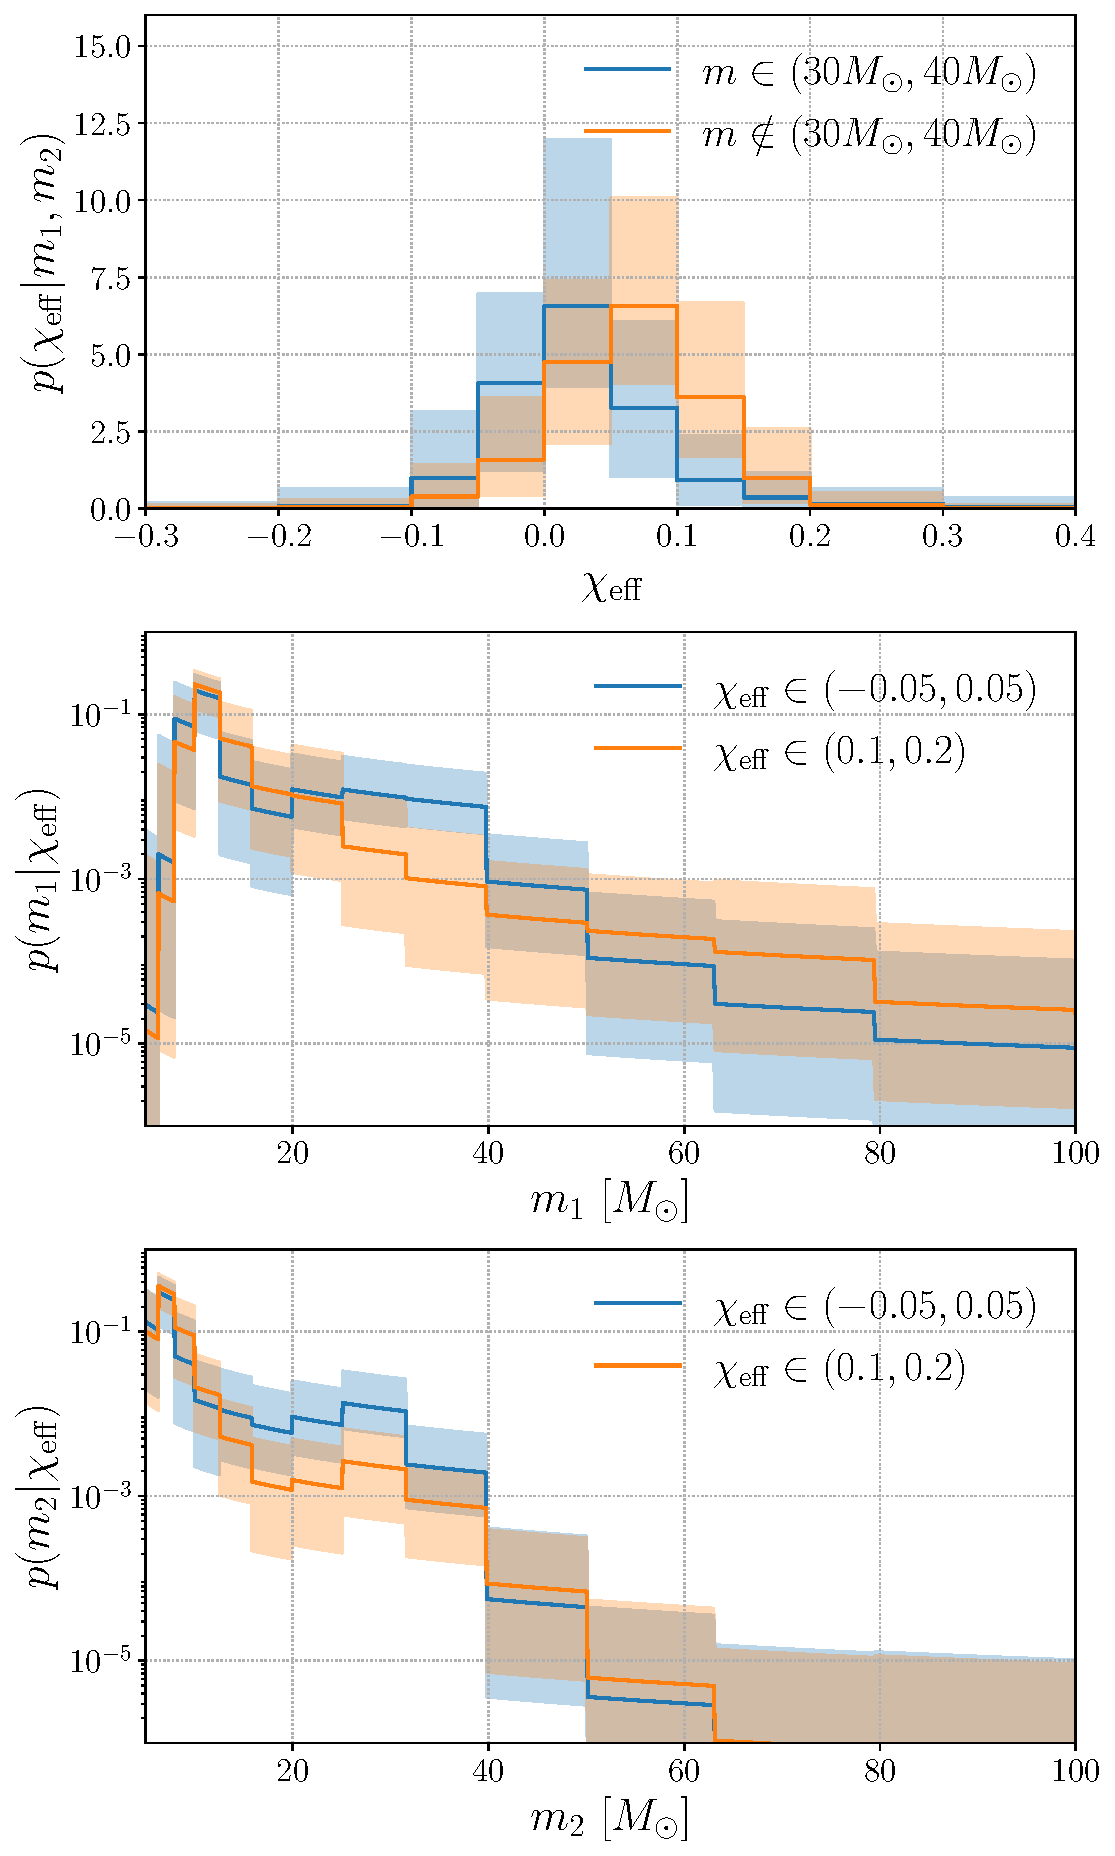
\includegraphics[width=0.5\columnwidth]{figures/mass_spin_correlated_bgp_combined.pdf}
	\caption{
  \textit{Top:} inferred distributions of effective inspiral spin $\chieff$ in the correlated mass--spin \ac{BGP}~analysis.
  The solid lines give the median, while the shaded regions indicate the \confidenceLevel~credible intervals.
  In blue, we have the $\chieff$ distribution of \ac{BBH} systems with at least one mass inside the $30{-}40 \,\Msun$ peak range.
	In orange, we have the $\chieff$ distribution of \ac{BBH} systems masses outside the $30{-}40 \,\Msun$ peak range.
  While the two distributions are consistent within \confidenceLevel~credible intervals, systems outside the peak range appear to favour a distribution of $\chieff$ skewed toward more positive values.
	Meanwhile, systems inside the peak range appear to favour a more symmetrical distribution about $\chieff = 0$.
  \textit{Middle:} inferred distributions of primary mass from the correlated mass--spin \ac{BGP}~analysis.
  \textit{Bottom:} inferred distributions of secondary mass from the correlated mass--spin \ac{BGP}~analysis.
	In both mass plots, blue shows the distribution for systems with small spins, $\chieff$ in the range $(-0.05,0.05)$, while orange shows the distribution for systems with larger spins, $\chieff$ in the range $(0.1,0.2)$.
	Note the preference for a higher proportion of mergers with masses $\approx 30{-}40 \,\Msun$ for low spin systems (blue).
	}
	\label{fig:mass_spin_correlated_bgp_combined}
\end{figure}

The \textsc{Isolated Peak}~model \citep[see also][]{Godfrey:2023oxb} fits the data to a model containing multiple mass subpopulations with independent spin distributions.
One subpopulation consists of a single peak in the mass distribution (which is inferred to center on ${\sim} 10 \,\Msun$), while other subpopulations are flexibly fit with the \BSpline~method.
Applying these analyses to \gwtcfour suggests that \acp{BH} within the ${\sim} 10 \,\Msun$ peak have a spin magnitude distribution consistent (within 90\% credibile intervals) with the rest of the \ac{BBH} population.
Meanwhile, although there is some overlap in the 90\% credibile regions of the cosine tilt distributions for both subpopulations, the distribution of tilts for \acp{BH} in the ${\sim} 10 \,\Msun$ peak favors alignment and is inconsistent with isotropy.
The distribution of cosine tilts for \acp{BH} outside this mass peak appears more symmetrical about $\cos \theta = 0$ and does not rule out isotropy.
Roughly speaking, this corresponds to a distribution of $\chieff$ that may be symmetrical about zero for the \ac{BBH} population outside of the ${\sim} 10 \,\Msun$ peak.
Inside this mass peak, however, the implied $\chieff$ distribution skews toward positive values.

We also model a correlation between primary mass and $\chieff$ using a copula model (see Appendix~\ref{appendix:copulaCorrelationModels}).
Fitting this \copulacorrelation~model with \gwtcfour data, we infer a correlation of $\kappa_{m_1, \mathrm{eff}} = \CIPlusMinus{\mchieffCopulaCorrelationModel[param][kappa]}$ between $m_1$ and $\chieff$.
Hence, the \copulacorrelation~analysis finds no evidence for a single, smooth, population-wide correlation between primary mass and $\chieff$.

Broadly, our analyses of the joint mass and spin distribution recover similar features to recent works that probe for features in \gwtcthree.
First, analyses of \gwtcthree do not find evidence for a smoothly correlated distribution in primary mass and $\chieff$ \citep{Safarzadeh:2020mlb, Biscoveanu:2022qac, Fishbach:2022lzq, Heinzel:2023hlb, Heinzel:2024hva, Antonini:2024het}, as is the case in this work.
Meanwhile, a number of analyses find evidence for separate subpopulations in mass and spin consistent with predictions of dynamical and field mergers.
More specifically, these works tend to find a subpopulation with lower masses and smaller, mostly aligned spins, and a second subpopulation of heavier binaries with larger, isotropically distributed spins, where the subpopulations transition around ${\sim} 40 \,\Msun$ \citep{Wang:2022gnx, Mould:2022ccw, Godfrey:2023oxb, Li:2023yyt, Antonini:2024het, Pierra:2024fbl, Guo:2024wwv, Li:2025rhu, Sadiq:2025vly}.
While the analyses presented in this work do not recover this exact feature (nor do they probe directly for it), the \textsc{Isolated Peak}~model's preference for aligned spins at ${\sim} 10 \,\Msun$ and isotropically distributed spins at higher masses may be related.

\subsubsection{Redshift and Spin Correlations}
\label{subsubsec:redshift_spin_correlations}
\textbf{We find evidence that the $\bm{\chieff}$ distribution broadens as redshift increases up to $\bm{z \sim 1}$}.
We again look for correlations between redshift and $\chieff$ by modeling the mean and width of the $\chieff$ distribution with a linear dependence on redshift (see Appendix~\ref{appendix:LinearCorrelationModels}).
\cite{Biscoveanu:2022qac} employed a \linearcorrelation~model for $(z,\chieff)$ to analyze \gwtcthree data, finding no evidence for redshift dependence in the mean of the $\chieff$ distribution, but suggesting that the $\chieff$ distribution broadens with increasing redshift ($\delta \ln \sigma_{\mathrm{eff}|z} > 0$ at 98.6\% credibility).
Updating this analysis to include \ac{O4a} data, we find more evidence for a broadening in the $\chieff$ distribution with redshift, with $\delta \ln \sigma_{\mathrm{eff}|z} > 0$ now inferred at $\zchieffLinearCorrelationModel[param][ln_sigma_chieff_1][percentile exclude zero]\%$ credibility.
The mean and width of the $\chieff$ distribution as functions of redshift are shown in Figure~\ref{fig:z_chieff_mu_sigma}.

The \splinecorrelation~model, which models the redshift dependence on the mean and width of the $\chieff$ distribution flexibly with cubic splines (see Appendix~\ref{appendix:SplineCorrelationModels}), is broadly consistent with the \linearcorrelation~model.
The exception is that the \splinecorrelation~model tends to recover the prior beyond a redshift of $z \gtrsim 1$.
This likely indicates that the \linearcorrelation~model is fitting a trend at low redshifts, then extending this trend to redshifts $z \gtrsim 1$ due to a lack of flexibility.
To further illustrate this point, the gray dashed line in Figure~\ref{fig:z_chieff_mu_sigma} indicates the redshift under which 90\% of the catalog's cumulative posterior support is contained.
Roughly speaking, this means our inferences above this redshift are informed by only ${\sim} 10\%$ of the data.
Therefore, while we find evidence that the $\chieff$ distribution broadens as binaries approach $z \sim 1$, we are unable to determine if this trend continues at higher redshifts.

We also model a correlation between redshift and $\chieff$ using a copula model, with variable correlation $\kappa_{z, \mathrm{eff}}$ (see Appendix~\ref{appendix:copulaCorrelationModels}).
In contrast to the above analyses, the \copulacorrelation~model finds evidence for a positive correlation in $(z,\chieff)$, inferring a value of $\kappa_{z, \mathrm{eff}} = \CIPlusMinus{\zchieffCopulaCorrelationModel[param][kappa]}$ (or $\kappa_{z, \mathrm{eff}} > 0$ with $\zchieffCopulaCorrelationModel[param][kappa][correlated percentile]\%$ credibility).
While the \copulacorrelation~model lacks the flexibility to fit a broadening directly, the long (albeit shallow) posterior tails reaching into both large-negative and large-positive values for $\kappa_{z, \mathrm{eff}}$ may relate to the broadening in the $\chieff$ distribution recovered by the \linearcorrelation~and~\splinecorrelation~models (see Appendix~\ref{appendix:supplementary_correlations}).
If the $z$-dependent broadening and constant mean of the $\chieff$ distribution from the \linearcorrelation~and~\splinecorrelation~models is to be believed, it is unclear why the posterior on $\kappa_{z, \mathrm{eff}}$ skews toward positive values, rather than being symmetric about zero.

\begin{figure}
  \centering
  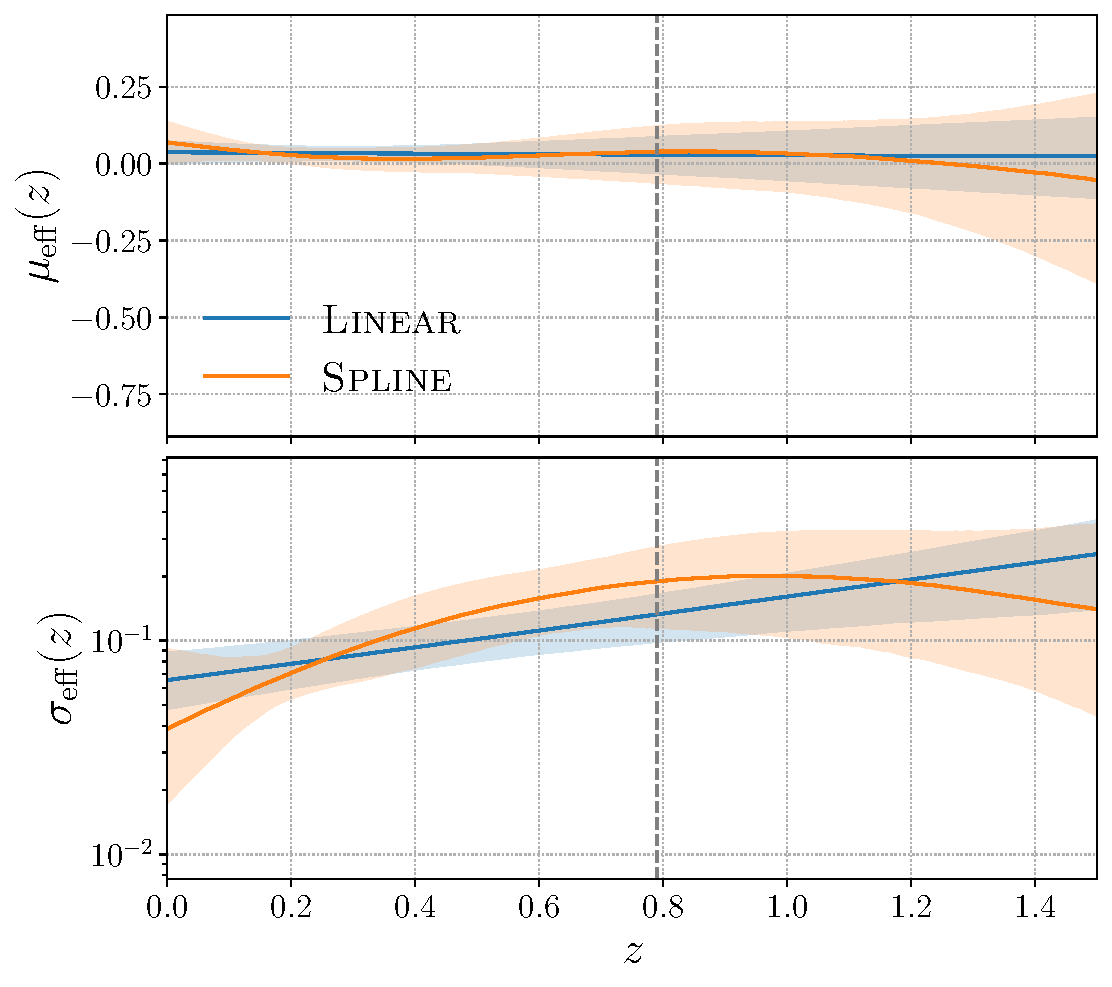
\includegraphics[width=0.6\columnwidth]{figures/correlation_spline_z_chi_eff.pdf}
  \caption{
  The inferred mean (top) and width (bottom) of the $\chieff$ distribution as a function of redshift for the \linearcorrelation~model (blue) and the \splinecorrelation~model (orange).
  The shaded regions give the \confidenceLevel~credible intervals.
  The gray dashed line indicates the redshift under which 90\% of the cumulative posterior probability lies across all events in \gwtcfour.
  Therefore, inferences above this redshift are dominated by the prior or population model.
  Note the logarithmic scale on the width (bottom panel).
  In either model, we find evidence that the width of the effective inspiral spin distribution increases with redshift up to $z \sim 1$.
  }
  \label{fig:z_chieff_mu_sigma}
\end{figure}

It is unclear what this broadening in the $\chieff$ distribution at greater redshifts might imply astrophysically.
Provided \ac{BH} progenitors experience significant spin up due to tidal torques, smaller orbital separations and periods will result in more efficient spin up of \ac{BBH} components \citep{Zaldarriaga:2017qkw, Mapelli:2018uds, Bavera:2020uch, Bavera:2022mef, Fuller:2022ysb}.
Of course, smaller orbital separations correspond to shorter delay-times to merger.
This means that these systems may contribute more to the merger rate in the earlier Universe (higher $z$), where systems with wider orbits have not had time to merge.
Furthermore, given that higher metallicity systems are expected to evolve to longer orbital periods due to experiencing more mass loss during core helium burning \citep{Qin:2018vaa, Fuller:2022ysb}, one might predict that larger spin magnitudes should be observed in regions of lower metallicity and thus also at higher redshifts.
However, the correlation in the \linearcorrelation~and~\splinecorrelation~models is between redshift and the width of the $\chieff$ distribution rather than the mean.
This includes an increasing number of systems with both large-positive and large-negative values of $\chieff$.
An increase in systems with large-negative $\chieff$ may be somewhat difficult to square with the above hypothesis, given that tidal spin up is only relevant in isolated systems, and that large supernovae kicks are required to misalign the \ac{BH} spins so significantly \citep{Kalogera:1999tq,  Wysocki:2017isg, Gerosa:2018wbw, Callister:2020vyz, Steinle:2020xej, Stevenson:2022hmi, Tauris:2022ggv, Baibhav:2024rkn}.
On the other hand, if the \copulacorrelation~results are to be taken at face-value, the preference for a positive correlation in $(z,\chieff)$ fits more neatly with the aforementioned hypothesis.

Another possibility, following discussion from Section~\ref{subsec:bbh_spins}, is that multiple separate subpopulations of \ac{BBH} mergers are being observed, where the more dominant (in terms of redshift-dependent merger rate) subpopulation changes at some nearby redshift.
Hierarchical mergers becoming more dominant at higher redshifts for example could potentially explain such a broadening in the effective spin distribution.
This interpretation would also imply some level of correlation between mass and redshift, which we do not find evidence for below in Section~\ref{subsubsec:redshift_mass_correlations}.

As a final caveat, using \gwtcthree data, \cite{Biscoveanu:2022qac} fit the \ac{BBH} population to a model in which the $\chieff$ distribution is linearly dependent on both primary mass and redshift.
In doing so, the authors find degeneracies between the $(m_1,\chieff)$ and $(z,\chieff)$ correlations.
While we do not explore correlations beyond two dimensions in this work, we acknowledge that the assumption of independence between other pairs of parameters may have notable effects on our inferences.

\subsubsection{Redshift and Mass Correlations}
\label{subsubsec:redshift_mass_correlations}
Finally, we consider potential correlations between BBH mass and redshift.
\textbf{We do not find evidence for evolution in the mass distribution with redshift.}
We emphasize that these inferences are constrained to the nearby Universe, with relatively little data beyond $z \sim 1$ (19 out of 153 \ac{BBH} events having posteriors consistent with $z>1$ to \confidenceLevel~credibility).
We model correlations between primary mass and redshift using a copula with correlation $\kappa_{m_1, z}$ (see Appendix~\ref{appendix:copulaCorrelationModels}).
Using this \copulacorrelation~model, we infer a correlation of $\kappa_{m_1, z} = \CIPlusMinus{\mzCopulaCorrelationModel[param][kappa]}$.
We also search for correlations between mass and redshift using a \ac{BGP}~analysis that allows for covariance in $m_1$ and $z$ (see Appendix~\ref{appendix:BGPModel}).
Similarly, this analysis finds that the mass distribution does not show a distinguishable evolution with redshift (see Appendix~\ref{appendix:supplementary_correlations}).
This conclusion is mostly in line with studies using \gwtcthree, which are also unable to infer any correlation between mass and redshift with confidence \citep{Fishbach:2021yvy, Sadiq:2021fin, vanSon:2021zpk, Karathanasis:2022rtr, Ray:2023upk, Heinzel:2023hlb, Heinzel:2024hva, Lalleman:2025xcs, Sadiq:2025aog}.
This is with the exception of \cite{Rinaldi:2023bbd} finding a positive correlation between \ac{BBH} primary mass and redshift, although a novel method is used to account for selection effects.

